%\documentclass[runningheads]{llncs}
\documentclass[]{llncs}
\usepackage{makeidx}
\usepackage{graphicx}
\begin{document}
\addtocmark{Southern Methodist University} % additional mark in the TOC

\title{LABORATORY EARTHQUAKE ANALYSIS}
%\subtitle{Optional Subtitle Goes Here}

\author{Olha Tanyuk\inst{1}, Daniel Davieau\inst{1}, Dr. Michael L. Blanpied\inst{2}, Dr. Charles South\inst{1} \and Dr. Daniel W. Engels\inst1}

\institute{Southern Methodist University, Dallas TX 75205, USA \and United States Geological Survey, Fort Worth, TX 76115}

\maketitle
%"Be careful not to accidentally plagurize"
% Do Not use figures from other publications. Even if you cite it; you are getting into areas where copyright issues arise.
% Write a clear engaging story
% Write in present tense
% No opinion words
%Define important words i.e Random Forest
%Short sentences
% Use tables instead of bullets - all bullets and lists should be tables.
% Visualizations should explain a lot. Viewer should get the point without having to read.

%Citations are always contained within the same sentence that they are citing, i.e., the citations come before the period ending the sentence – preferably right next to the words needing to be cited



%%%%%%%%%%%%%%%%%%%%%%%%%%%%%%%%%%%%%%%%%%%%%%%%%%%%%%%%%%%%%%%%%%%
%In Draft Two, you will continue to use the given template, and you will have made significant progress in documenting, in well-polished prose and figures and tables, the tutorial material, related work, solution approach, data, early results, analysis of those results, ethics, and early conclusions. 
%%%%%%%%%%%%%%%%%%%%%%%%%%%%%%%%%%%%%%%%%%%%%%%%%%%%%%%%%%%%%%%%%%%

%%%%%%%%%%%%%%%%%%%%%%%%%%%%%%%%%%%%%%%%%%%%%%%%%%%%%%%%%%%%%%%%%%%%
%Abstract draft 2 should be well written with placeholder sentences for the main result and main conclusion if early results and conclusions have not been obtained already. 
%%%%%%%%%%%%%%%%%%%%%%%%%%%%%%%%%%%%%%%%%%%%%%%%%%%%%%%%%%%%%%%%%%%%
% Abstract Structure:
%	Problem sentence
%	Motivation Sentence
%	2=3 what you did to solve the problem
%	1 sentence main result(singular with a number)
%	1 sentence main conclusion (singular)
\begin{abstract}
In 2017 the Los Alamos National Laboratory (LANL) conducted an experiment which predicted the remaining time before {\em laboratory} earthquakes occured with .89 coefficient of determination\cite{Bertrand}. LANL has since collected additional data with considerably more a-periodic laboratory earthquake failures and made it available to the public in 2019.

Can laboratory earthquakes be predicted more accurately given this considerably more a-periodic data?

In this {\em new} study we apply machine learning to analyze patterns in the a-periodic data. We design statistical models to predict the remaining time before laboratory earthquakes occur.  We compare predicted versus actual time remaining to determine our accuracy.\par

The result proves that impending laboratory earthquakes can be predicted with {\em(TBD coefficient of determination)}. The predictions are based solely on the characteristics of recorded acoustical signals; they are not based on time intervals between prior laboratory earthquakes.\par



\end{abstract}
\section{INTRODUCTION}
%%%%%%%%%%%%%%%%%%%%%%%%%%%%%%%%%%%%%%%%%%%%%%%%%%%%%%%%%%%%%%%%%%%%%%%%
%The Introduction section should be written with draft paragraphs for the results and conclusions. The Introduction should be 2 to 4 pages in length in the given format. Remember that both the Abstract and the Introduction are executive summaries of your work.
%%%%%%%%%%%%%%%%%%%%%%%%%%%%%%%%%%%%%%%%%%%%%%%%%%%%%%%%%%%%%%%%%%%%%%%%
%INTRODUCTION
%1 Paragraph Motivtion (Sets Genreral problem domain)
%1 Paragraph P{roblem Statement (Specific Problem solved by the work)
%2-3 paragraphs on solution
% 1 Paragraph on main results (plural)
% 1 Paragraph on main conclusions (plural)
% 1 Paragraph on paper organization

Earthquakes cause mass destruction and loss of life. A traditional method to predict earthquakes is to look to past recurrence intervals. Because the recurrences are not constant, predictions can only be made within broad time windows.\par 

In August 2017 the Los Alamos National Laboratory (LANL) conducted an experiment\cite{Bertrand} which predicted \emph{laboratory} earthquakes with 90\% accuracy. The team imitated an earthquake using steel blocks interacting with rocky material to induce slipping that emitted seismic signals. An accelerometer was used to record them. A random forest algorithm was trained on the signals and stick‐slip failures (laboratory earthquakes). The trained algorithm was then used to generate predictions from separate signals (not used in the training). The predictions were measured against actual failures to determine the accuracy of the predictions\cite{LANLNews}.\par

\begin{quote}“Over the last 15 years, there has been renewed hope that progress can be made regarding forecasting owing to tremendous advances in instrumentation quality and density\cite{Bertrand}."\end{quote}

There have been improvements in the technology used to measure and collect laboratory seismic signal data. LANL has collected additional data and made it available to the public for a 2019 Kaggle competition. \par

\begin{quote}
	“For this challenge we selected an experiment that exhibits a very a-periodic and more realistic behavior compared to the data we studied in our early work, with earthquakes occurring very irregularly\cite{kaggle}." 
\end{quote}

\begin{quote}
	“If this challenge is solved and the physics are ultimately shown to scale from the laboratory to the field, researchers will have the potential to improve earthquake hazard assessments that could save lives and billions of dollars in infrastructure\cite{kaggle}."
\end{quote}

There have also been improvements in computing capabilities. There are now publicly available software packages Keras, Tensorflow, Nvidia CUDA™ and Turing™ GPU architecture. These improvements enable us to apply complex deep learning algorithms which were more difficult or impossible to employ in the past.\par

%Problem Statement
Given seismic signal data with considerably more a-periodic laboratory earthquake failures, improved computing hardware and software can we improve on the Los Alamos study\cite{Bertrand} to determine when laboratory earthquakes will occur?\par

%Solution
In this {\em new} observational study we employ a series of algorithms and predict impending laboratory earthquakes with {\em (additional facts to be gathered)} accuracy.

%Conclusion
The a-periodic data, hardware and software allows us to predict impending earthquakes more accurately. However we only know 8-16 seconds before failure. Therefore practical applications may be limited. This may prove useful but only applies to laboratory experiments. {\em (How to collect data for real world earthquakes?)}  This could be used in industry perhaps researching materials for wallboard, machine parts.\par

\section{TUTORIAL MATERIAL}
%%%%%%%%%%%%%%%%%%%%%%%%%%%%%%%%%%%%%%%%%%%%%%%%%%%%%%%%%%%%%%%%%%%%%%%%
%Draft Two should include all of the tutorial sections in well-written nearly polished form. Your paper is targeted at a general technical audience (think – students who are just beginning the MSDS program, but have not yet taken any classes in the program, except the Stats Bridge and the Programming Bridge). Therefore, background sections on your problem domain are necessary for all readers to be able to properly understand your work.
%%%%%%%%%%%%%%%%%%%%%%%%%%%%%%%%%%%%%%%%%%%%%%%%%%%%%%%%%%%%%%%%%%%%%%%%
%Paper should be tutorial in nature
%Audience is data scientists of varying levels of knowledge. Keep newer students in mind
We hear about earthquakes usually via news media when there is a large seismic event which is noticeable and causes death and destruction. These are stick–slip events that radiate seismic energy along the faults between tectonic plates. In this study we refer to these as {\em Regular Earthquakes}. Regular earthquakes are caused by a sudden slip on a fault. Tectonic plates move slowly but can get stuck at their edges due to friction. Stress builds gradually over time until it overcomes the friction resulting in a slip between the tectonic plates. Energy is released in waves that travel through the earth's crust. This is the shaking that we feel and know as an earthquake\cite{USGSfaqs}.\par

Another type of earthquake we refer to in this study is a {\em Slow Slip Earthquake} (SSE). SSE's are fault behaviors that occur slowly enough to make them undetectable without instrumentation. They do not shake the ground and cause widespread destruction like regular earthquakes do. They occur near the boundaries of large earthquake rupture zones\cite{Slip}. \par

LANL researchers discovered a way to predict earthquakes in a laboratory experiment that simulates natural conditions. In 2017 they discovered a way to train a computer to pinpoint and analyze seismic signals emitted during movements along faults to predict an earthquake. They processed massive amounts of data and identified a particular sound pattern previously thought to be just white noise that preceded an earthquake. The team was able to characterize the time remaining before a laboratory earthquake at all times\cite{LANLNews}. \par

%In the lab, the team imitated a real earthquake using steel blocks interacting with rocky material (fault gouge) to induce slipping that emitted seismic sounds. An accelerometer recorded the acoustic emission emanating from the sheared layers[6].\par

For the first time they discovered a pattern that accurately predicted when a laboratory earthquake would occur. The team acknowledged that the physical traits of the lab experiment differ from the real world but the application of the analysis to real earthquakes to validate their results is ongoing. This method can also be applied outside of seismology to support materials’ failure research in many fields such as aerospace and energy\cite{LANLNews}.\par

The results revealed that the faults failed in a predictable manner. The observations also demonstrated that the fault’s critical stress state can be determined using exclusively an equation of state\cite{LANLNews}.\par

Traditionally scientists have relied exclusively on historical data to  characterize the state of faults and predict regular earthquakes. Only a small fraction of seismic data had typically been collected and some was discarded during analysis as noise. The LANL team discovered that hidden in this noise are signals emitted by the fault that inform them of the state of the fault much more precisely\cite{LANLNews}.\par
\begin{quote}
“Our work shows that machine learning can be used to extract new meaningful physics from a very well studied system,” said Bertrand Rouet-Leduc, Los Alamos Earth and Environmental Sciences Division scientist and the paper’s lead author. “It also shows that seismogenic faults are continuously broadcasting a signal that precisely informs us of their physical state and how close they are to rupture, at least in the laboratory.”
\end{quote}

This suggests that there is a relationship between slow slip earthquakes and more noticeable regular earthquakes\cite{SlowSlip}. This study analyzes the relationship between slow slip and regular earthquakes. We use this relationship information to predict regular laboratory earthquakes. \par


\section{DATA} The data used in this study was provided by LANL's 2019 Kaggle competition\cite{kaggle}. It was collected using a three-block assembly with two gouge layers placed in a bi-axial stress configuration. Two 5mm thick fault gouge layers were placed between the three blocks, which were held in place by a fixed normal load. The gouge material was comprised of beads with diameter 105-149 mm. The central block was sheared at constant displacement rate. The two data streams recorded were the shear stress and the acoustic signal. While the gouge material was in a critical shear stress regime, the shear stress abruptly dropped which indicated gouge failure(a laboratory earthquake). As applied load progressively increased, the recurrence of laboratory earthquakes progressively decreased. At smaller applied loads the slips became a-periodic. The acoustic particle acceleration was measured on the central block.\par

LANL is certain the signal recorded for analysis is the acoustic signal emanating from the fault\cite{Bertrand}.\par

The data is 157.275 seconds of seismic data recorded at 4MHz hence 629,143,480 observations. Each observation is accompanied by a record of the time remaining before the next laboratory earthquake occurred. The observations are a continuous segment. The seismic signals are signed integer values ranging from -5515 to 5444. The time to failure recordings are floating point decimal ranging from {\em min max} in seconds. \par

\begin{figure}[h]
	\centering
	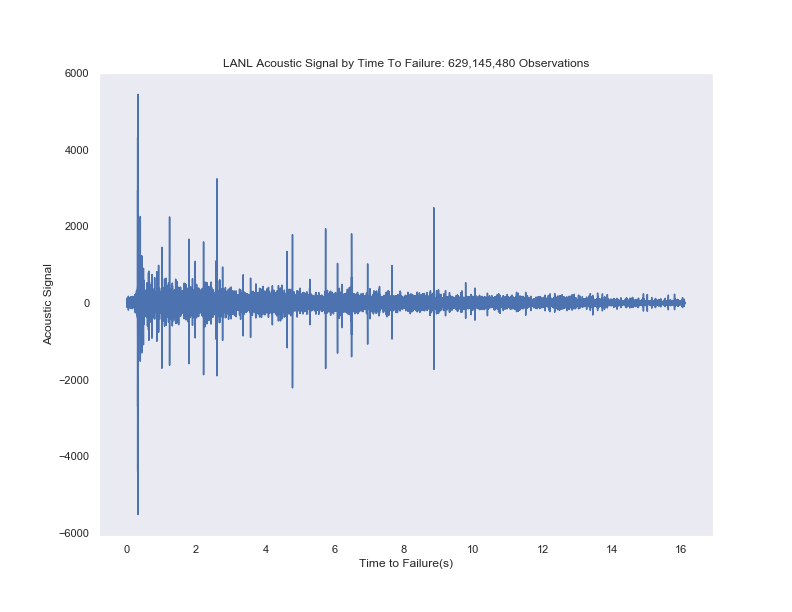
\includegraphics[width=1\linewidth]{../GPUProject/allDataDefaultPlot}
	\caption{The magnitude of each seismic signal and the time remaining before the next laboratory earthquake. There are 16 lab earthquakes. The shortest time to failure is 1.5 seconds for the first earthquake and 7 seconds for the 7th, while the longest is around 16 seconds.}
	\label{fig:alldatadefaultplot}
\end{figure}
\begin{table}[h!]
	\begin{center}
		\caption{Sample of Data Provided}
		\label{tab:table1}
		\begin{tabular}{l|c|r} 
			\textbf{Index} & \textbf{Seismic Signal} & \textbf{Time to Failure}\\
			\hline
			0 & 12 & 1.469099998474121 \\ 
			1 & 6 & 1.469099998474121 \\ 
			2 & 8 & 1.469099998474121 \\ 
			3 & 5 & 1.469099998474121 \\ 
			4 & 8 & 1.469099998474121 \\ 
		\end{tabular}
	\end{center}
\end{table}
\begin{figure}
	\centering
	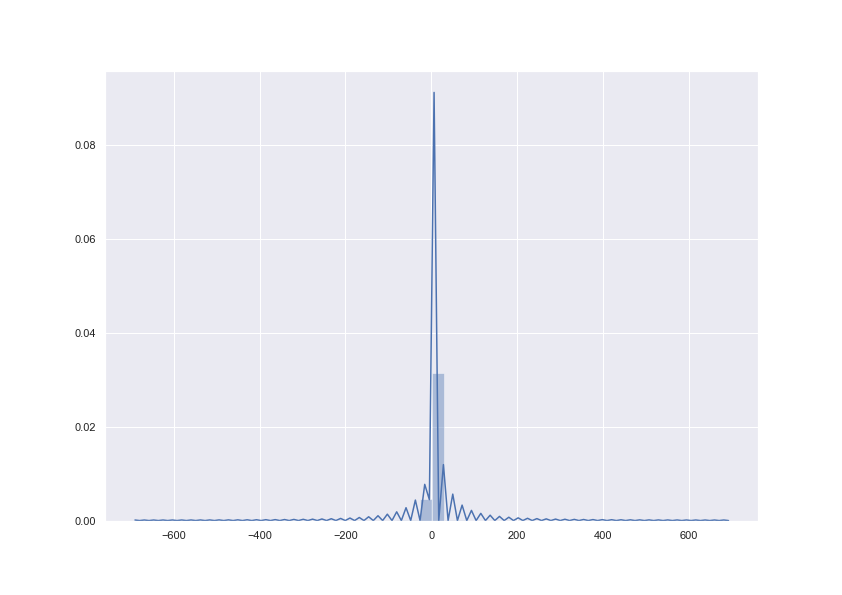
\includegraphics[width=.8\linewidth]{../GPUProject/acousticRand60000DistPlot}
	\caption{The distribution of seismic signal measurements by LANL}
	\label{fig:acousticRand60000DistPlot}
\end{figure}
The acoustic data are integers ranging from -5515 to 5444 and have mean of 4.52. The time to failure is in seconds. We can see that acoustic data shows large fluctuations just before the failure and recurs cyclically. Failures can be predicted visually as cases when huge fluctuations in the signal are followed by smaller signal values. This could be useful for predicting time to failure changes from 0 to high values.
\begin{figure}[h]
	\centering
	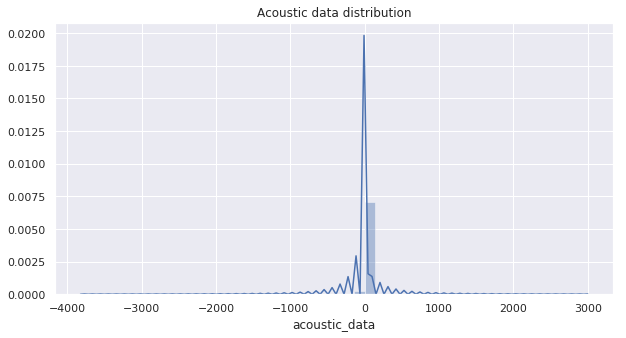
\includegraphics[width=0.7\linewidth]{../GPUProject/acousticFeatureIntegers}
	\caption[]{1\% random sample from 629,143,480 observations}
	\label{fig:acousticfeatureintegers}
\end{figure}



\begin{table}[h!]
	\begin{center}
		\caption{Seismic Signal Stats}
		\label{tab:table1}
		\begin{tabular}{l|c} % <-- Alignments: 1st column left, 2nd middle and 3rd right, with vertical lines in between
			\textbf{Index} & \textbf{Seismic Signal} \\
			\hline
			count &  6.29145480\\ 
			mean & 4.47708428 \\ 
			std &  2.61278939\\ 
			min &  9.55039650\\ 
			25 & 2.62599707 \\ 
			50 &  5.34979773\\ 
			75 &  8.17339516\\ 
			max & 1.61074009 \\ 
		\end{tabular}
	\end{center}
\end{table}
\begin{figure}[h]
	\centering
	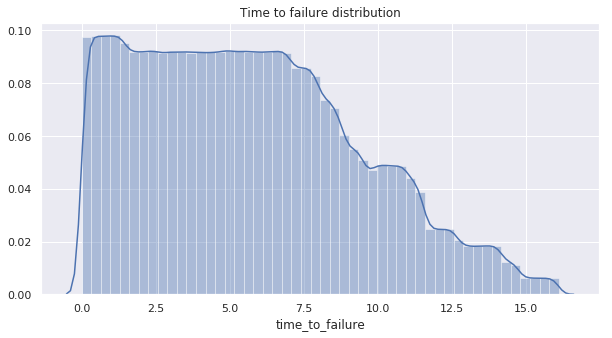
\includegraphics[width=0.7\linewidth]{../GPUProject/timeToFailureDistribution}
	\caption[]{The min value is very close to zero and the max is 16 seconds.}
	\label{fig:timetofailuredistribution}
\end{figure}



\begin{figure}[h]
	\centering
	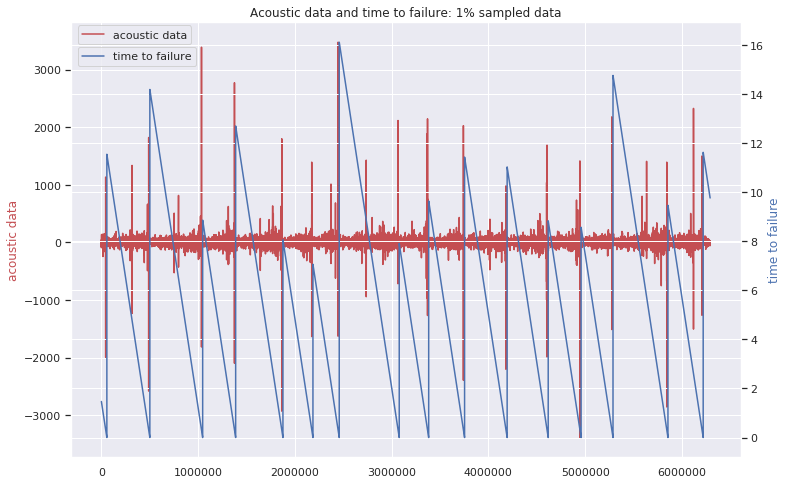
\includegraphics[width=0.8\linewidth]{../GPUProject/timeSeries}
	\caption{We checked how both variables changed over time. The red line is the acoustic data and the blue one is the time to failure. On a plot above we can see, that training data has 16 earthquakes. The shortest time to failure is 1.5 seconds for the first earthquake and 7seconds for the 7th, while the longest is around 16 seconds.}
	\label{fig:timeseries}
\end{figure}

\begin{figure}
	\centering
	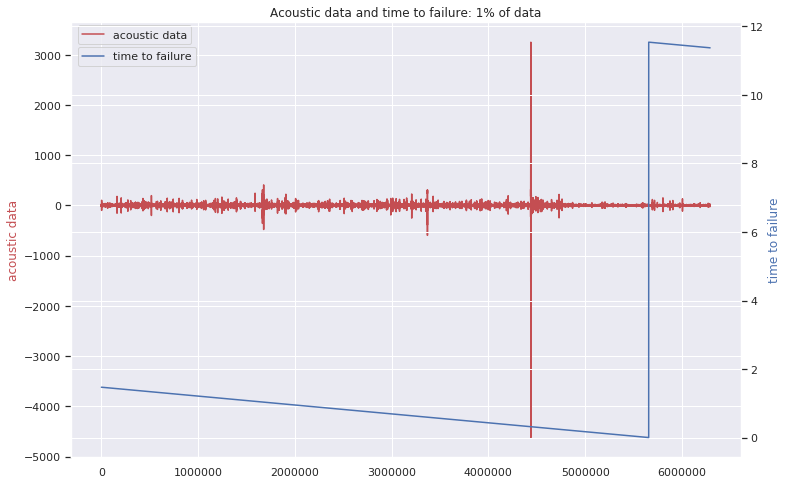
\includegraphics[width=0.7\linewidth]{../GPUProject/zoomedInTimePlot}
	\caption{On this zoomed-in-time plot we can see that actually the large oscillation before the failure is not quite in the last moment. There are also trains of intense oscillations proceeding the large one and also some oscillations with smaller peaks after the large one. Then, after some minor oscillations, the failure occurs. Interesting thing to check is the time between high levels of seismic signal and the earthquakes. We are considering any acoustic data with absolute value greater than 1000 as a high level}
	\label{fig:zoomedintimeplot}
\end{figure}

\begin{figure}
	\centering
	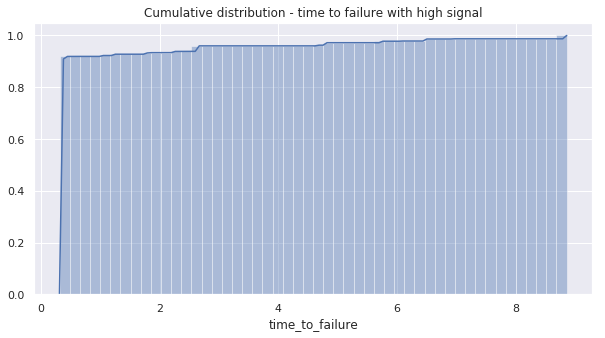
\includegraphics[width=0.7\linewidth]{../GPUProject/moreThan90percent}
	\caption{More than 90\% of high acoustic values are around 0.31 seconds before an earthquake}
		\label{fig:morethan90percent}
	\end{figure}

\section{METHODS AND EXPERIMENTS}
% Describe the solution approach here.
% Define algorithms, methods and experiments
% DO NOT give play by play of everything we did
% Don't put code in paper; if anything put in appendix.
% Put versions of software but no one cares about how to use technology; just state what we did.

Our goal is to predict the time remaining before the next failure using only moving time windows of the acoustic data. We divided our data by windows that contains 150,000 observations each (0.0375 seconds of seismic data), so our new data set is 4194 windows. From each time window, we compute a set of 98 potentially relevant statistical features (e.g., mean, variance, kurtosis). 
We apply a machine learning techniques such as the Random Forest Regressor, XGB Regressor,  Decision Tree Regressor, LGBM Regressor, Extra Trees Regressor to the new continuous values that we got, analysing acoustic time series data.\par
Similarly to the LANL study we created new features can be separated into two main classes: 
Distribution of signal’s energy: we use couple of higher order moments of the acoustic data to capture the evolution of the signal’s energy. Within each time window we compute the signal’s normalized mean, minimum, maximum and higher moments  (variance, skewness, kurtosis).\par
Precursors: the system enters a critical state when close to failure. We rely on different percentiles and thresholds to monitor this precursory activity. We use the 1st - 9th and 91th - 99th percentiles. Our thresholds measure the count of observations that the acoustic signal spends over a threshold value f0 and under a threshold value f1.

In order to avoid correlation between new features we applied principal component analysis.  Instead of using 98 features, we created just 10 that represented 99.9% of the full data variation.
We use a 70/30 random split of the full time series for use as training and testing data sets respectively. We computed regularization hyper-parameters for each machine learning predicting techniques by random grid search based on a 3-fold cross-validation.
\subsection{Data Transformations}
The distribution of time to failure is right skewed. We apply a square root transformation to normalize it and improve the prediction models. It is still not ideally normal, but looks much more better after the transformation.
\begin{figure}
	\centering
	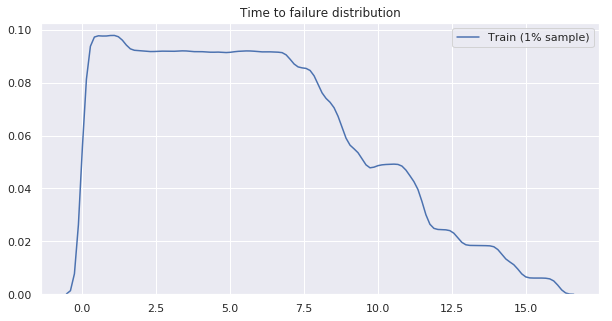
\includegraphics[width=1\linewidth]{../GPUProject/transform1}
	\caption{Distribution of Time to Failure showing right skew}
	\label{fig:morethan90percent}
\end{figure}

\begin{figure}
	\centering
	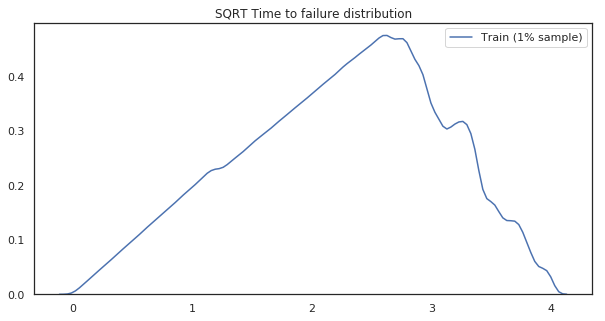
\includegraphics[width=1\linewidth]{../GPUProject/transform2}
	\caption{Distribution of Time to Failure showing improved normality after applying square root}
	\label{fig:morethan90percent}
\end{figure}





\subsection{Algorithms}
\subsection{Recursive Neural Network}
LSTM is a type of RNN that helps us deal with vanishing or exploding gradients (incorrect slope). For example most of our acoustic signal observations are within x however more extreme signals occur just before failure. The extreme differences between these observations can skew the accuracy of more traditional RNN algorithms.

LSTM separates the long term(fault slip) from short term (slow slip)
Hidden state= memory from prior observations
Typical RNN input+priorhiddenstate>tanh (-1,1) activation function>new hidden state
LSTM is same but includes gates to determine what information is included in hidden state and what is not.

The gates are rnn's themselves.

input+priorhiddenstate>sigmoid (0,1) activation function>new hidden state. 0, 1 allows us to forget or remmeber 
Patrick Yam: LSTM cannot handle data with 150000 sequence length therefore we wavenet in the earlier layers as feature extraction and reduce the sequence length to 150.\par

Forget gate decides what to include 1, or exclude 0. 
https://www.youtube.com/watch?v=2GNbIKTKCfE
https://www.youtube.com/watch?v=8HyCNIVRbSU

\subsection{Auto Regressive integrated Moving Average (ARIMA)}
The data shows evidence of non-stationarity (the mean, variance change over time). We use an ARMIA model to analyze the changing means and variance. This this model also can also account for white noise.\par ARIMA(0,0,0)

\subsection{Gradient Boosting Decision Tree}

%http://mlexplained.com/2018/01/05/lightgbm-and-xgboost-explained/
%mean absolute error: 2.230923263623967
%r2 score: 0.42923076680297423

\section{RESULTS}
%Include evaluation methodology
%Use tables and graphs
%Don't forget explanations

We run 5 different techniques on a train data set (70 percent of the full data) before principal component analysis and after. Principal component analysis did not improve our findings significantly, that is why we are not represent those results here. For each model we provide hyper-parameters details for future reproducibility (Table 2).
When making a prediction (red curve), we emphasize that there is no past or future information considered: each prediction uses only the information within one single time window of the acoustic signal. We quantify the accuracy of our model using R2 (the coefficient of determination) and MAE (mean absolute error), applying predicting model on a 30 percent of the full data (test data).


%It is clear that the LSTM + Wave-net algorithms %are superior performers.
%This is because it handles extreme variations in the slope (gradient descent) and we can tune it to remember not only the common signals but the extreme signals which occur only when failure is imminent.
%Use tables and graphs
%Use tables and graphs
%Use tables and graphs
%Don't forget explanations

\begin{figure}
	\centering
	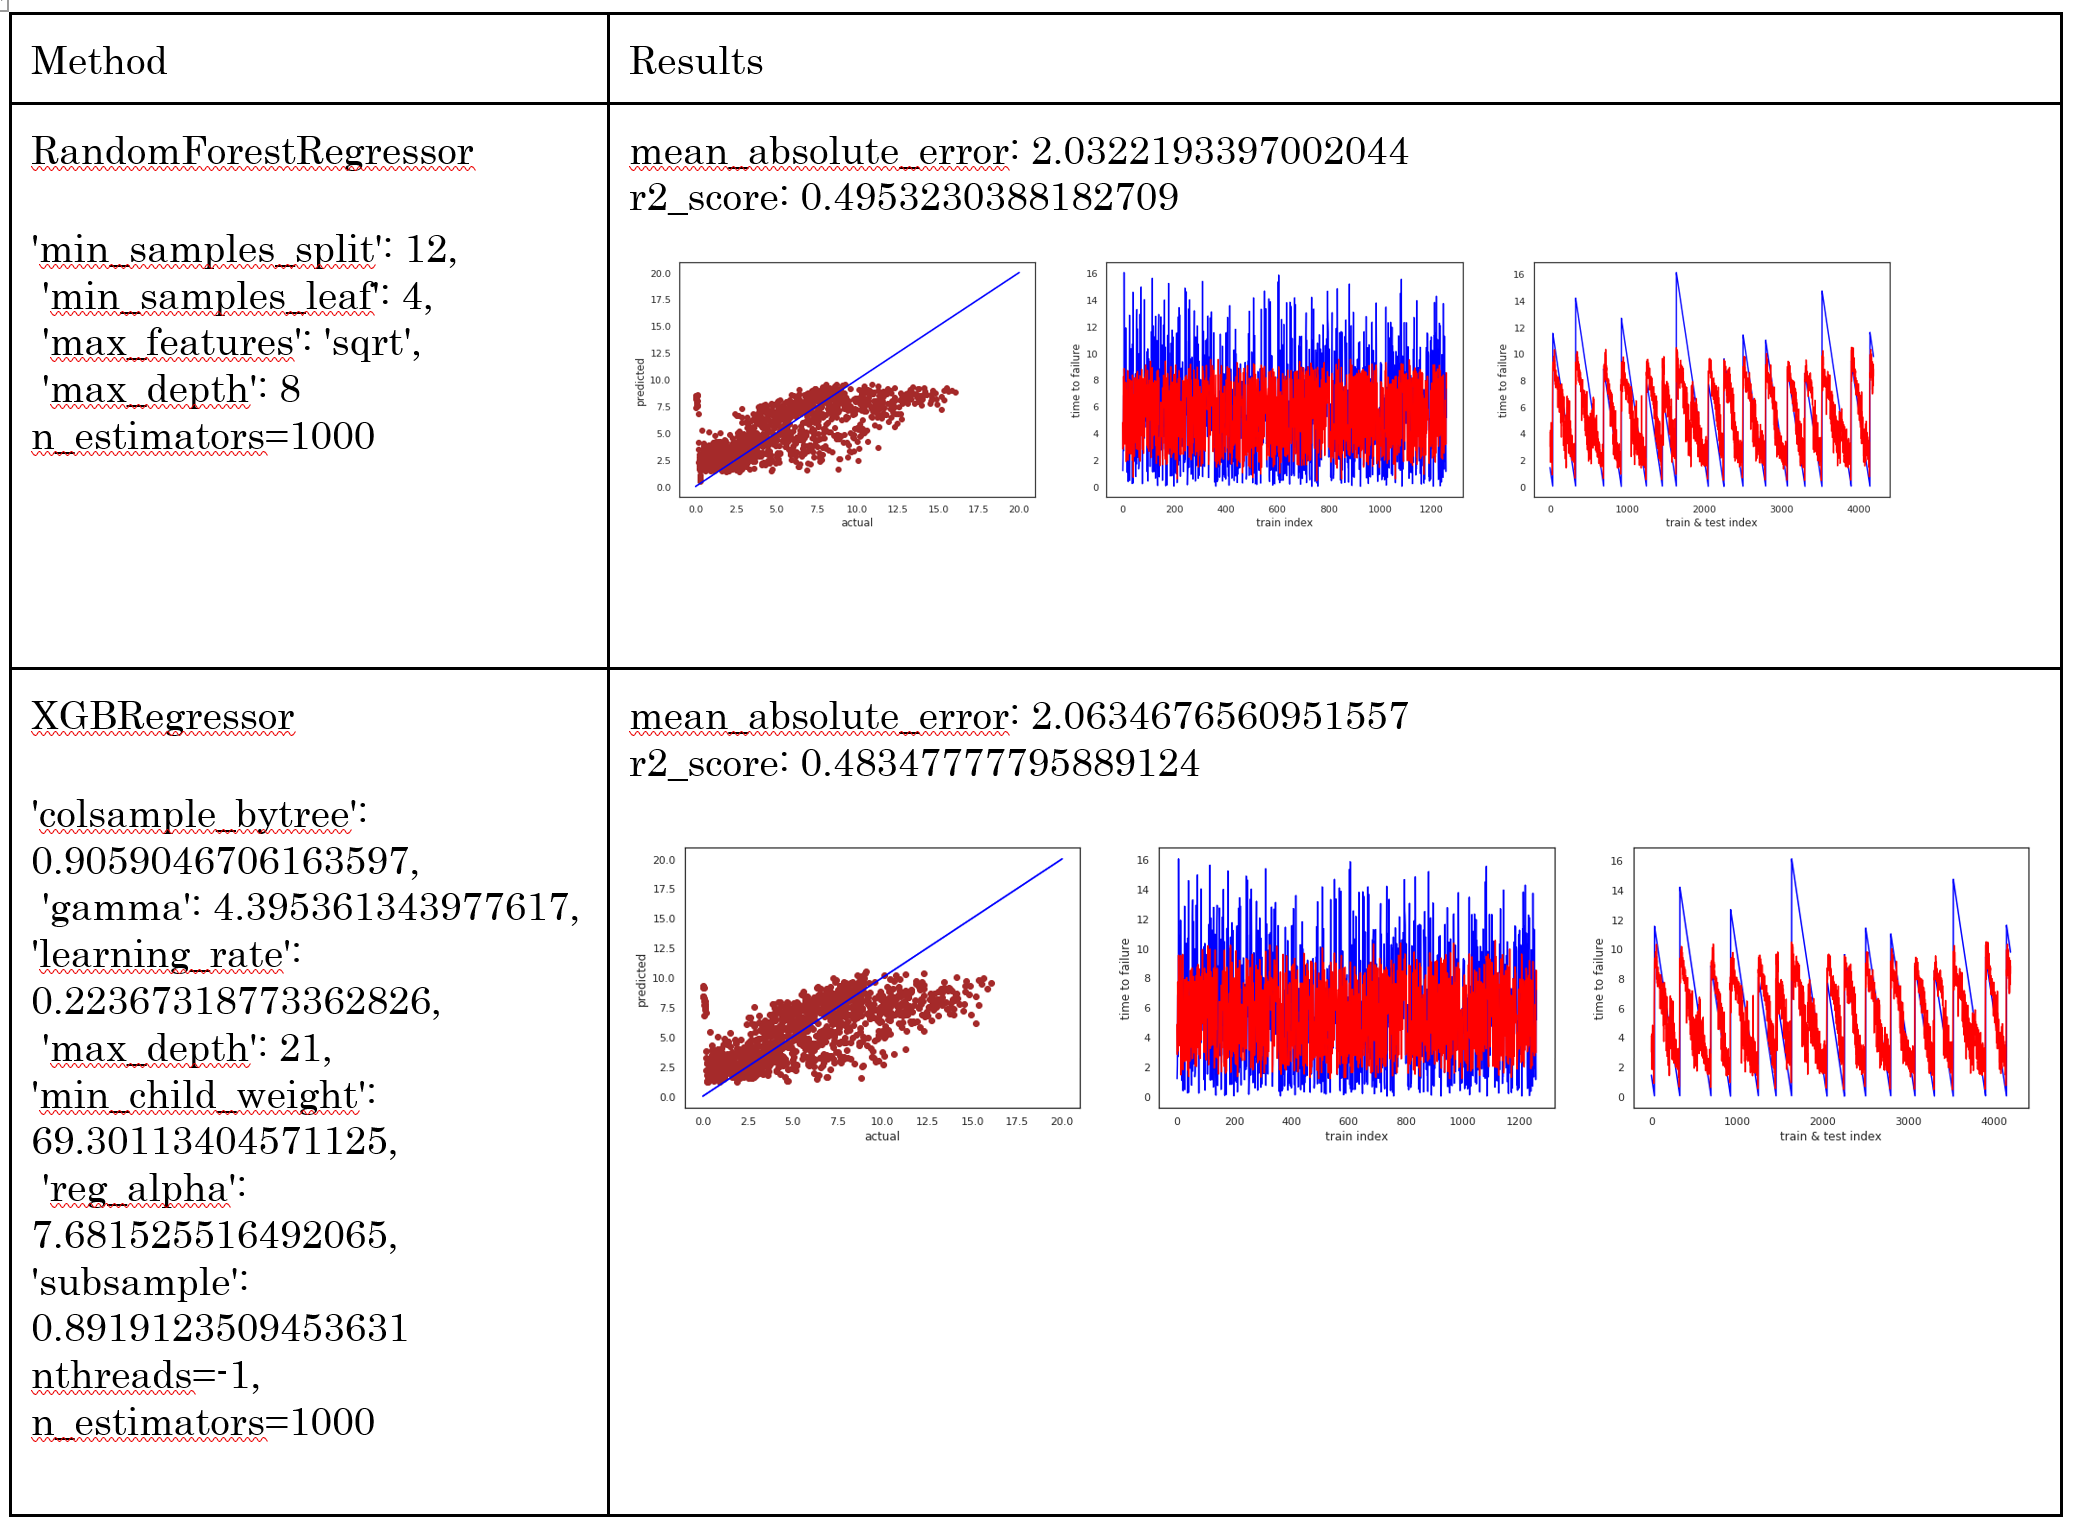
\includegraphics[width=1\linewidth]{../GPUProject/Results1.PNG}
	\caption{Results by Model}
	\label{fig:morethan90percent}
\end{figure}

\begin{figure}
	\centering
	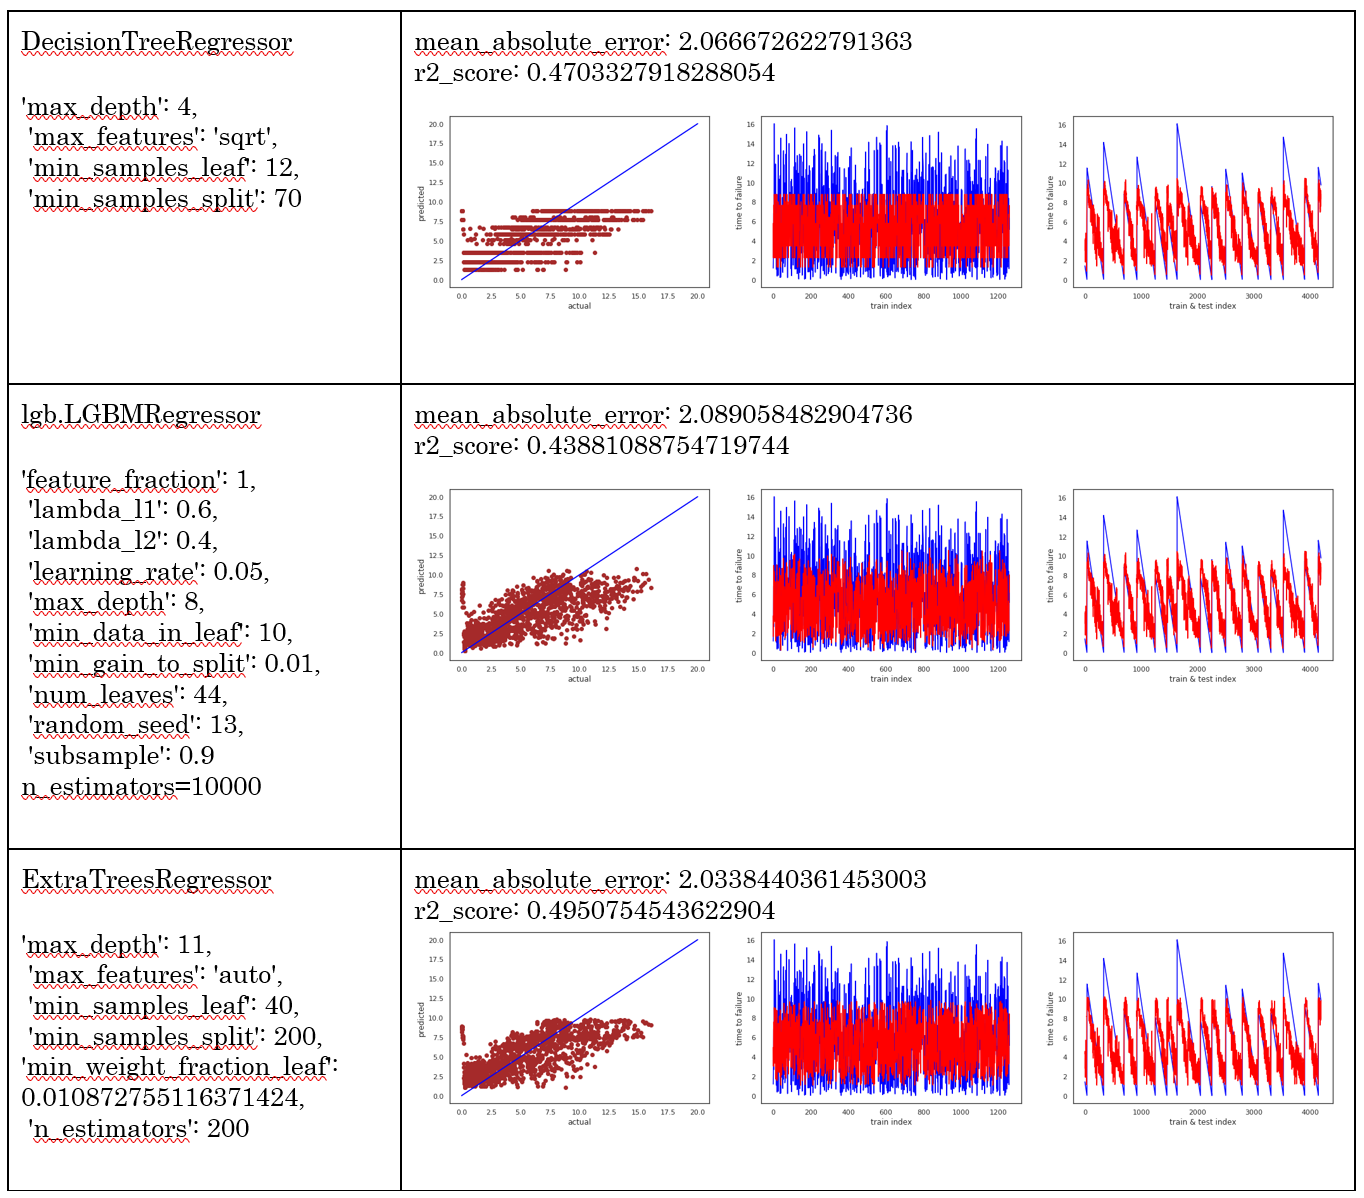
\includegraphics[width=1\linewidth]{../GPUProject/Results2.PNG}
	\caption{Results by Model}
	\label{fig:morethan90percent}
\end{figure}

\section{ANALYSIS}
The most accurate results with coefficient of determination 0.5 and mean absolute error 2.03 we got using Random Forest Regressor. The most important features, shown on Fig. 7, suggest to check our data for correlated features, since rolling standard deviations show the same patterns. Plus in order to improve our predicting model, we need to get rid of features that have importance equal to 0 or close to 0, such as hypermoment, minimum, maximum and some of the rolling means. Currently we are working on improving of the model to make prediction for the beginning and the end of the one quake cycle. As you can see on a Fig. 1, seismic waves with small voltage are in our interest. Random forest model accurately predicts failure across load level, but hardly can predict outliers. It means that we still need to think about new features that we missing. Precursors that we choose during feature engineering were not good enough when the system enters a critical state close to failure.
\begin{figure}
	\centering
	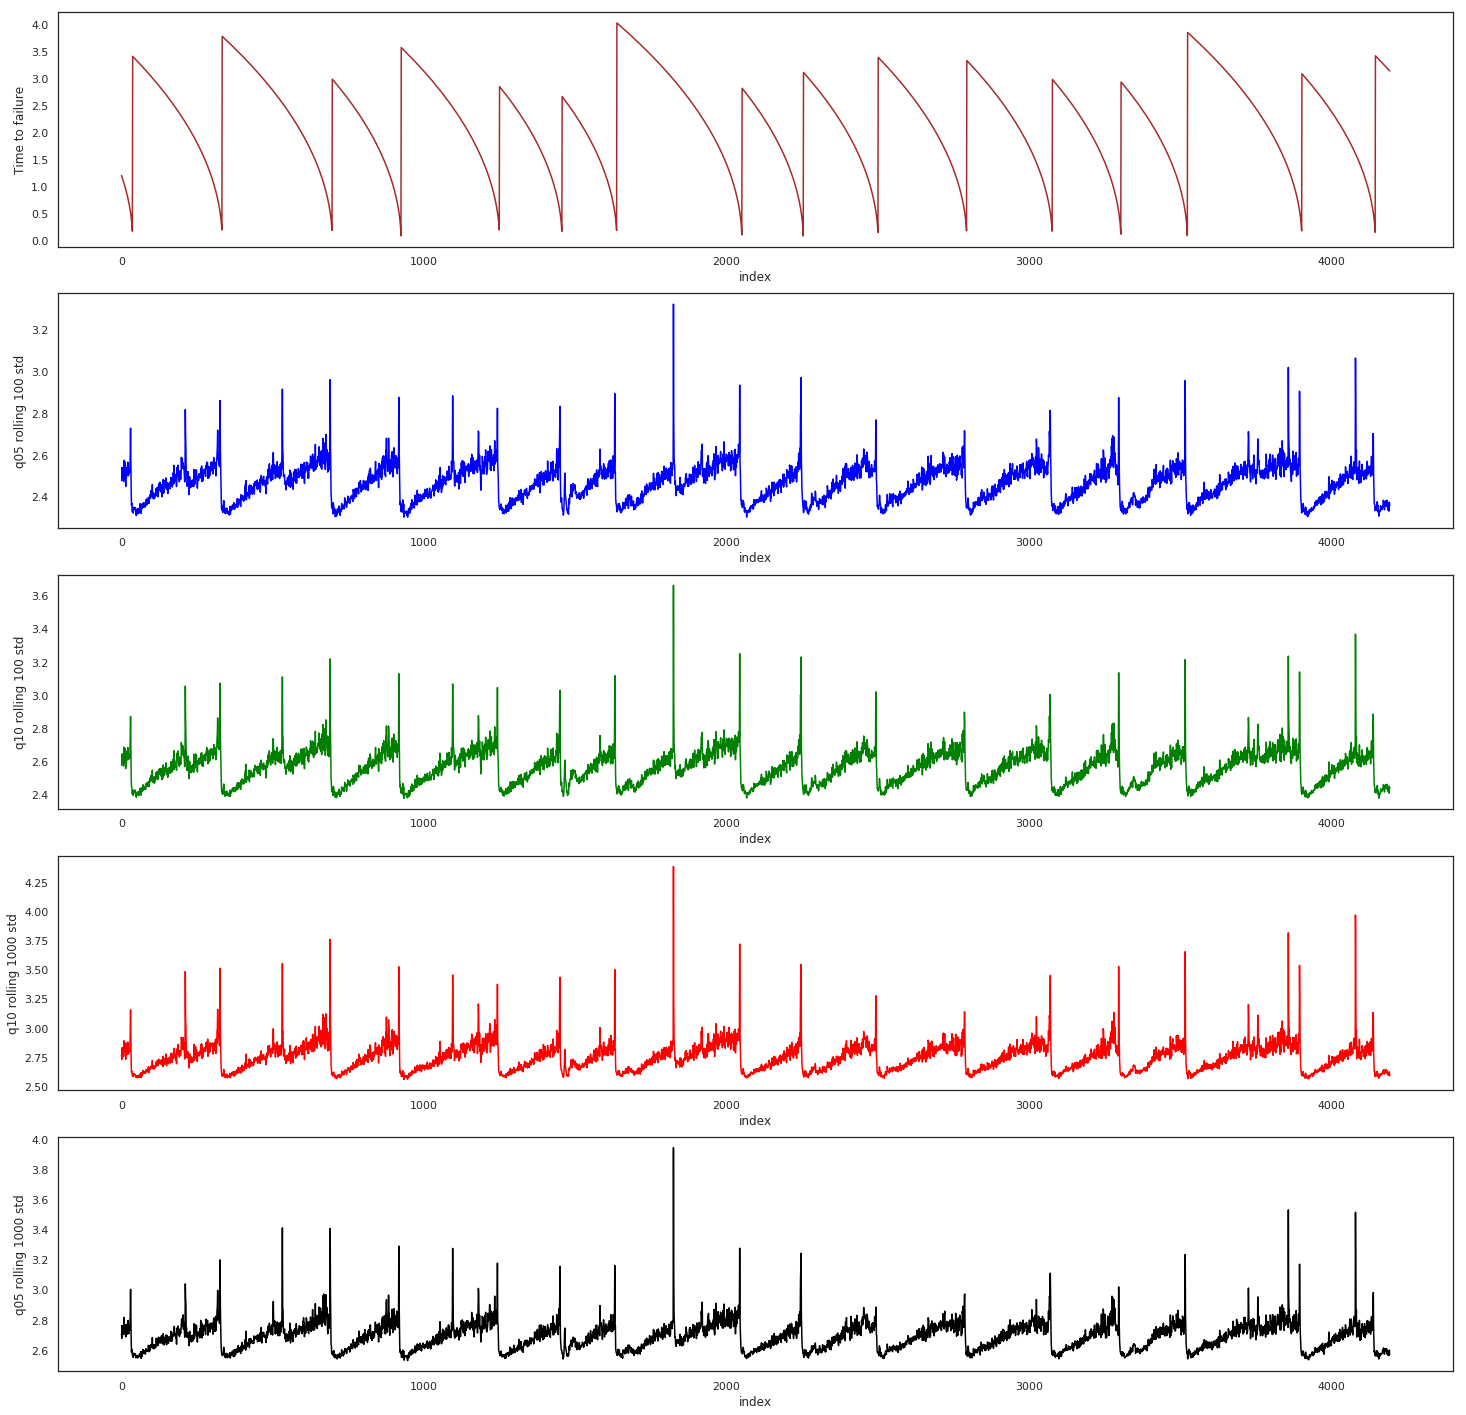
\includegraphics[width=1\linewidth]{../GPUProject/Analysis1.png}
	\caption{Predictions by Model}
	\label{fig:morethan90percent}
\end{figure}

\section{ETHICS}
If people believe us and we are wrong; bad things can happen. If people believe us and we are right; good and bad things can happen.

Scientists’ responsibility to inform the public about their results may conflict with their responsibility not to cause social disturbance by the communication of these results. A study of the well-known Brady-Spence and Iben Browning earthquake predictions illustrates this conflict in the publication of scientifically unwarranted predictions. Furthermore, a public policy that considers public sensitivity caused by such publications as an opportunity to promote public awareness is ethically problematic from (i) a refined consequentialist point of view that any means cannot be justified by any ends, and (ii) a rights view according to which individuals should never be treated as a mere means to ends\cite{Ayhan}.


\section{CONCLUSION}
{\em Draw a minimum of 3 conclusions  This is NOT a summary section.} 
\par

The evidence in this new {\em observational} study suggests that {\em (Measure against prior study TBD. We have to state the fact that we cannot prove that the data collection technology improvements are better or that our algorithm is better unless we can accurately reproduce the prior model's results. Consider confounding variables such as different collection methods and unavailable details about the 2017 model.)}\par

We are able to predict with Mean absolute Error = 0.5680 however we  only know 8-16 seconds before failure.
 Therefore practical applications may be limited. This may prove useful but only applies to laboratory experiments. 
 
 Our application of machine learning predicts failures with 2.03 seconds mean absolute error and 0.5 coefficient of determination. This is based on the analysis of the acoustic signal every moment in the slip cycle. 
 
 Machine learning searches for patterns that humans may not easily perceive. This method may be useful if LANL can scale it from the lab to the field. It can also be useful in researching industrial and natural materials.
 
 
 
 
\par

\bibliographystyle{splncs}
\bibliography{OlgaDan}
\end{document}
